\chapter{The Question}
\label{ch:32}



\begin{center}
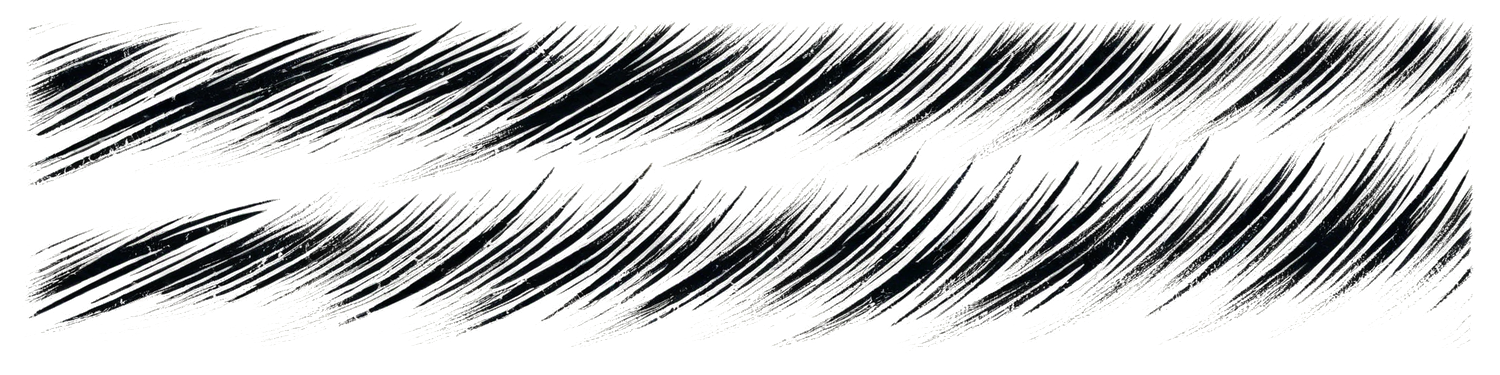
\includegraphics[width=\textwidth]{images/chapterImages/genesis_sketch_00133_.png}
\end{center}

The documentary crew took three hours to set up. Lights. Cameras. Sound equipment. Too much equipment for one elderly woman sitting in her living room answering questions about discoveries made fifty years ago. But this was the big interview. The definitive statement. Dr. Sarah Chen, at seventy-six years old, finally speaking comprehensively about the genetic programming of humanity.

She'd refused interviews for decades. Let other people talk. Let younger researchers analyze and debate and philosophize. She'd done her work. Translated the message. Published the data. Then retreated to Montana to live out her years in the small house Marcus had built before he died.

But Nathaniel had asked her to do this. "People need to hear from you, Grandma. Not the theories. Not the interpretations. Your experience. What you learned. What you still don't know."

So here she was. Seventy-six years old. Thirty years since Maya died—cancer, sudden, brutal. Twenty-five years with Marcus before his heart stopped one morning while he was building a chair. Ten years alone in this house watching humanity spread to Mars, Europa, three moons of Saturn.

Ten years watching new activation sequences express. Terraforming capability. Deep space navigation. Quantum consciousness expansion—whatever that meant. The program continued. The thresholds kept coming. The equation unfolded.

"Dr. Chen, are you ready?" The interviewer was young. Thirty, maybe. Born after the revelation. Grew up knowing she was executing code. It showed in her body language—less existential crisis, more pragmatic acceptance.

"Ready," Sarah said.

The cameras started. Lights brightened. The interviewer smiled professionally.

"Dr. Chen, fifty years ago you discovered that human evolution was programmed by intelligent dinosaurs. That every major capability—from tool use to space travel—was encoded into our DNA 65 million years ago. Can you describe what that moment of discovery felt like?"

Sarah thought about it. The real question beneath the question. How did it feel to learn nothing was what it seemed? How did it feel to prove humanity was executing code?

"Terrifying," she said. "Devastating. Like everything I thought I knew about being human was wrong. Like free will was an illusion. Like my choices weren't mine."

"And now? Fifty years later? Do you still feel that way?"

"I don't know. Some days yes. Some days no. Some days I think the question is wrong."

The interviewer leaned forward slightly. This was what she'd come for. Not the history. The ambiguity. The uncertainty. The fact that even Sarah Chen, after fifty years, didn't have a clean answer.

"What do you mean the question is wrong?"

"We ask 'Do we have free will?' But maybe that's not one question. Maybe it's a thousand questions. Do I choose what I'm capable of? No. That's programmed. Do I choose what I'm compelled toward? Unclear. Probably not. Do I choose how I respond to the compulsion? Maybe. Do I choose what I do with the capability? Sometimes. Do I choose whether to accept or resist? That's the complicated one."

"Can you elaborate?"

Sarah looked out the window. The Montana landscape. Mountains. Trees. The workshop Marcus had built still standing. The furniture he'd made still functional. Pointless, unnecessary furniture that he'd chosen to create even knowing choice might be illusion.

"There was an engineer," Sarah said. "Woman named Dr. Patterson. Activated for planetary defense like thousands of others. But she decided to resist. Thought if the compulsion was genetic, she could overcome it with willpower. Went off-grid. Tried to suppress the activation through meditation, drugs, sensory deprivation. Lasted three months. Then had a psychotic break. Never recovered fully. Died still believing she could have resisted if she'd just tried harder."

"Was she right?"

"I don't know. The compulsion is biological. It's real. It's overwhelming. Most people can't resist and don't try. But a few have managed to redirect it. To channel the drive toward different applications. Same capability, different implementation. Is that choice? Or just variation in how the code executes?"

The interviewer checked her notes. "You wrote in your 2055 paper that 'The program provides capacity, not destiny. The genetics determine what we can do, not what we must do.' Do you still believe that?"

"I believe it some days. Other days I think I was being optimistic. Trying to preserve the illusion of autonomy."

"Which interpretation is correct?"

"How would I know? If I'm programmed to believe I have choice, how could I tell whether I actually have choice? The program could include the feeling of free will without the reality of it. Could include self-awareness of programming without the ability to override it."

Sarah saw something flicker across the interviewer's face. Discomfort. The question everyone carried around like a weight. If we're programs, what does that make us? What does that make anything?

"Let me ask differently," the interviewer said. "Your personal life. Your relationship with your daughter. With Marcus Chen. With your grandson. Did those feel programmed?"

Sarah smiled slightly. "All of it. None of it. Both simultaneously."

"Can you explain?"

"Maya hated me for years. Rightfully. I was activated for research capability and I couldn't override it. Couldn't choose her over the work. That was programming. But later—after I translated the message—I made an effort. Showed up. Tried to repair things. Was that choice? Or was that just the next phase of the program? A subroutine for relationship maintenance once primary function was complete?"

"What do you think?"

"I think it felt like choice. I think I wanted to do it. But I also think the wanting might have been programmed. The need to connect with Maya might have been biological imperative. Social bonding to ensure genetic lineage continuation. I can't separate the programming from the person because I'm not sure there's a separation."

"And Marcus Chen?"

Sarah was quiet for a moment. Even after ten years, thinking about Marcus was complicated. Twenty-five years together. Building furniture and watching the stars and trying to figure out if love was real or just chemical recognition.

"Marcus believed that choosing to accept the programming made it real. That even if our feelings were biological, the decision to act on them was valid. That authenticity wasn't about freedom from code—it was about choosing which code to execute."

"Did you agree?"

"I didn't have a better theory."

The interviewer smiled. Actually smiled, not the professional version. "My partner is activated for terraforming. She's compelled to go to Mars next year. Work on atmospheric modification. She'll be gone for at least a decade. Maybe forever. We're trying to decide whether to stay together. Whether long-distance love is meaningful if it's just biology managing separation anxiety."

"What will you do?"

"I don't know. She says she loves me. I believe her. But I also know the activation is affecting her neurochemistry. Changing how she processes emotion. Making the work more appealing than the relationship. Is that her choosing her career? Or is that programming overriding her connection to me?"

"What does she say?"

"That she doesn't know. That she wants to stay. That she wants to go. That both are true. That she can't tell what she feels versus what she's compelled to feel."

Sarah nodded. "That's the question. That's always the question."

"And you never found an answer."

"I found twelve answers. All contradictory. All simultaneously true."

The interviewer laughed. Almost crying. The sound of someone who'd been carrying this weight alone and just realized other people carried it too.

"Does it get easier?" she asked. Off script now. Just asking.

"No," Sarah said. "But you get used to it. The uncertainty. The confusion. The not knowing. You realize that maybe humans never knew if they had free will. Maybe this question is as old as consciousness. Maybe the dinosaurs asked it too, in their way. Maybe every being that thinks asks whether thinking is real or just processes executing."

"What do you think Aurelia would say? If we could ask them?"

Sarah thought about this. About Aurelia standing in the canyon calculating. The Companion dying. The work continuing. The message encoded in DNA: *Pass it forward. 0.14\% is better than zero.*

"I think they'd say it doesn't matter. I think they'd say the work needs doing regardless of whether the worker is free. I think they'd say love—if that's what they felt—was real enough that they acted on it. Built a future for it. Died for it. Whether they were compelled or chose to be compelled is philosophical distinction. The action was the same."

"Is that enough? Action without certainty about volition?"

"It has to be. It's all we have."

The interviewer looked down at her notes. Regrouped. Returned to script. "Dr. Chen, there are currently seventeen known activation thresholds. We've passed twelve of them. Five more are coming. One of them—the quantum consciousness expansion—some researchers believe might actually allow us to perceive whether we're programmed or not. To see the code from outside it. Do you think that's possible?"

"I think if it's programmed, we'll perceive what the program wants us to perceive."

"So we can never know."

"Probably not."

"Doesn't that bother you?"

Sarah thought about Maya's funeral. Marcus dying. Nathaniel having children of his own. Watching generations live and die while the program continued executing. Watching humanity spread to other worlds while the central question remained unanswered.

"It bothered me for thirty years. Consumed me. Made me obsessive. Made me destroy relationships trying to find certainty. Then one day Marcus said something. He was building a rocking chair for Nathaniel's daughter. My great-granddaughter. He said, 'I don't know if I'm choosing to build this. But I'm building it for someone I love. If that's programming, it's good programming.'"

"Was that enough for you?"

"No. But it helped. Made me realize that maybe the question isn't 'Am I free?' Maybe the question is 'What am I building? Who am I building it for? Does the thing I'm making add something to the world?' The motivation might be programmed but the creation is still real."

"You're saying we should stop asking whether we have free will?"

"I'm saying we won't get an answer. So we might as well ask different questions. Better questions."

"Like what?"

"Like 'What did Aurelia give us?' Like 'How do we use it well?' Like 'What do we pass forward?'"

The interviewer was quiet for a moment. Then: "Your grandson, Nathaniel, just published a paper suggesting that the entire activation sequence is designed to turn humanity into what the dinosaurs were. That we're becoming the next version of them. Inheriting not just their capability but their purpose. Do you agree with that theory?"

Sarah smiled. Nathaniel had always seen patterns others missed. Like her. Like Katherine. Like everyone activated for mathematical reasoning.

"It's a good theory. Makes sense. We're building what they couldn't build. Protecting what they couldn't protect. Continuing what they couldn't continue. We're their future. Their children, in a genetic sense. Children always inherit from their parents."

"Does that make the programming less invasive? Knowing it's inheritance?"

"I don't know. Does it matter whether your genes come from parents or from intentional design? Either way they determine so much. Either way you didn't choose them. Either way you're executing instructions written before you existed."

"But we know who wrote ours. We know why."

"Yes. That's different. That's huge. Knowing Aurelia loved us enough to die for us. Knowing they saw 0.14\% chance and took it anyway. Knowing they worked while grieving. Knowing they chose—if they chose—to build something for beings they'd never meet. That changes how I think about the programming."

"How?"

"Makes it feel less like control. More like gift. Doesn't make it freedom. But makes it... meaningful? Intentional? I don't know the right word."

"Love?"

Sarah looked at the young woman. The interviewer who was trying to decide whether to stay with her partner. Who was asking the same questions Sarah had asked fifty years ago. Who would probably never get better answers.

"Yeah," Sarah said. "Maybe love. Weird mathematical 65-million-year-old dinosaur love. But love."

"Do you think that's really love? Or is that just... I don't know... programming that looks like love?"

"I've been asking that question for fifty years. About Aurelia and The Companion. About me and Maya. About me and Marcus. About every feeling I've ever had."

"And?"

"And I still don't know. But Marcus is dead. Maya is dead. Aurelia and The Companion have been dead for 65 million years. And I still feel something when I think about them. Still miss them. Still grateful for what they gave me even when I'm angry about what it cost. If that's programming, it's convincing programming."

"Is convincing enough?"

"It has to be. It's all I can verify."

The interviewer looked at her notes again. Last question coming. Sarah could feel it. The big one. The reason they'd come.

"Dr. Chen, after fifty years of living with this knowledge, after decades of research, after losing and finding and losing again—do you think we have free will?"

Sarah looked out the window again. The Montana landscape. The workshop. The furniture. The life she'd built after the compulsion released her. The grandson who visited weekly. The great-grandchildren who asked questions about dinosaurs and programming and whether love was real.

The question she'd been asking since she was forty-eight years old and discovered the activation sequences.

The question she still couldn't answer.

"I don't know," she said. "Some days I think yes—the program gives capacity but we choose implementation. Some days I think no—everything is determined and choice is illusion. Some days I think the question is meaningless because we're embedded in the system and can't see outside it. Some days I think free will is something that emerges from the programming rather than existing separate from it. Some days I think I'm free when I accept the compulsion and imprisoned when I resist it. Some days I think the opposite."

"So... you don't know."

"I don't know. After fifty years. After all the research. After all the loss and discovery and grief and understanding. I don't know."

"Does that bother you?"

Sarah smiled. Really smiled. The first genuine smile in the entire interview.

"No," she said. "Not anymore. I spent thirty years torturing myself trying to know. Trying to find certainty. Trying to separate programming from choice. And I couldn't. No one can. But I can live with uncertainty. Can accept that some questions don't have answers. Can build furniture and love my grandson and miss my daughter and remember Marcus without knowing whether any of it was real or programmed or both or neither."

"That's your final answer? After everything? 'I don't know'?"

"That's my final answer. And I think it's the only honest answer anyone can give. We're conscious programs trying to figure out if consciousness is real or just emergent behavior from complex programming. We're asking whether the observer is separate from the observed while being the observed. It's a paradox. Maybe an unsolvable one."

"So we should just... stop asking?"

"No. We should keep asking. Keep investigating. Keep trying to understand. That's what Aurelia gave us. Curiosity. The drive to understand. The compulsion to analyze and calculate and discover. That might be programming but it's good programming. It's the thing that makes us human. Or the thing that makes us the dinosaurs' children. Same thing, maybe."

The interviewer signaled to her crew. Interview complete. Cameras off. Lights down. The documentary would probably edit this into something more profound. More certain. More satisfying than "I don't know."

But "I don't know" was the truth.

After they left, Sarah sat in her living room watching the light fade. Thinking about Aurelia. About Maya. About Marcus. About Nathaniel and his children and the great-grandchildren who carried the same code modified 65 million years ago.

The program was still executing. Still unfolding. Still passing capability forward.

And Sarah Chen, having spent fifty years trying to understand it, had finally made peace with mystery.

Had finally accepted that some questions don't have answers.

Had finally learned that uncertainty was okay. That "I don't know" was enough.

That 0.14\% was better than zero.

And that was enough too.

The sun set over Montana. The workshop cast shadows. The furniture Marcus built still stood.

And Sarah Chen, the woman who discovered humanity was programmed, sat in the gathering dark and felt something she chose to call peace.

Whether that choice was real or programmed, she didn't know.

Didn't need to know.

Not anymore.

The equation was still unfolding.

The program was still executing.

The inheritance was still passing forward.

And that was enough.

